% Tento soubor nahraďte vlastním souborem s obsahem práce.
%=========================================================================
% Autoři: Michal Bidlo, Bohuslav Křena, Jaroslav Dytrych, Petr Veigend a Adam Herout 2019


\chapter{Úvod}
\label{uvod}

\chapter{Teorie}
\label{teorie}
Cílem této kapitoly je seznámit čtenáře s koncepty nutnými pro pochopení vlastního řešení. Kapitola vysvětluje co je to voxel a jaká jsou jeho hlavní využití v počítačové grafice. Dále popisuje fotorealistické zobrazování a vykreslování voxelových scén obecně. Jsou zde popsány často používané akcelerační struktury pro vykreslování voxelových modelů.

\section{Realistické zobrazování}
Tato sekce popisuje princip a použití různých technik realistického zobrazování používaného v současné počítačové grafice. Jsou zde uvedeny pouze relevantní informace související s tématem a předpokládá se znalost základních termínů.

Realistické zobrazování je podle knihy \cite{gfx_principles_practice} definováno jako tvoření obrazu podle definovaného modelu scény a osvětlení v ní přítomné. Jednotlivé pixely ve vytvořeném snímku (anlg. rendered image) se dají chápat jako množství světla procházejícího podél paprsků ve scéně; to odpovídá integrálu vstupující světelné energie v bodě, případně v regionu.

Dle knihy \cite{real_time_render}, základní komponentou zobrazování v počítačové grafice je zobrazovací řetězec (angl. rendering pipeline). Funkcí zobrazovacího řetězce je vygenerování dvourozměrného snímku daného virtuální kamerou, scénou obsahující vykreslované modely a zdroji světla.

V článku \cite{render_eq} je představena zobrazovací rovnice. Je to integrální rovnice, jež zobecňuje přenos světelných paprsků ve scéně. Rovnice je ve tvaru

\begin{equation} \label{eq:render}
	\begin{gathered}
		I(x, x') = g(x, x') \Big[\varepsilon(x, x') + \int_S\rho(x, x', x'')I(x', x'')dx''\Big]
	\end{gathered}
\end{equation}

kde $I(x, x')$ je intenzita světla z bodu $x'$ do bodu $x$, $g(x, x')$ je geometrický term reprezentující zastínění povrchu mezi body $x$ a $x'$, $\varepsilon(x, x')$ značí intenzitu emitujícího světla z bodu $x'$ do bodu $x$ a $\rho(x, x', x'')$ představuje intenzitu rozptýleného světla z bodu $x''$ do bodu $x$ přes plochu povrchu $x'$. Integrál je vypočten přes $S = \bigcup S_i$, tedy jako sjednocení všech povrchů, kdy $S_0$ je dostatečně velká hemisféra uzavírající celou scénu.

Jak je dále uvedeno v článku \cite{render_eq}, rovnice vychází z fyzikální rovnice radiozity. Popisuje přenos intenzity světla z jednoho povrchového bodu do jiného jako sumu emitovaného osvětlení a celkové intenzity rozptýleného světla v bodě $x$ od všech okolních povrchových bodů.

Podobná zobrazovací rovnice byla představena souběžně se dříve zmíněnou rovnicí v článku \cite{render_eq_2}. Tato rovnice je popsána pomocí vektorů a je v literatuře používána častěji. Nejznámější formu zobrazovací rovnice popisuje kniha \cite{gfx_principles_practice}:

\begin{equation} \label{eq:render_2}
	\begin{gathered}
		L_{out}(P, \omega_0) = L_e(P, \omega) + \int_{\omega_i\in S^2(p)}L_{in}(P, -\omega_i)f_s(P, \omega_i, \omega_0)(\omega_i \cdot \textbf{n}_P)d\omega_i
	\end{gathered}
\end{equation}
kde $L(P, \omega)$ je příchozí ($L_{in}$) či odchozí ($L_{out}$) světlo v bodě $P$ ve směru $\omega$, $\textbf{n}_P$ je normála povrchu v bodě $P$, $\omega_i$ značí příchozí směr světla, $\omega_0$ analogicky odchozí směr světla a $S$ je sjednocení všech povrchů. $L_{out}$ je světlo vyzářené pryč z bodu $P$ ve směru $\omega_0$ (tedy směrem k pozorovateli), $L_e$ je emitované světlo, $L_{in}$ je světlo přicházející z $\omega_i$ a $f_s$ je obousměrná distribuční funkce odrazu světla (BRDF)(světlo odražené z $\omega_i$ k $\omega_0$).

Existuje mnoho metod realistického zobrazování, následuje základní popis vybraných.

\subsection{Ray tracing}
Nebo sledování paprsku. Pravděpodobně nejznámější metoda globálního osvětlení. Kniha \cite{advanced_global} popisuje ray tracing jako algoritmus počítající radianční hodnotu $L_{pixel}$ pro každý pixel ve výsledném obrázku. Tato hodnota je váženou hodnotou osvětlení ve scéně obsaženou v cestě paprsku:

\begin{equation} \label{eq:rt_1}
	\begin{gathered}
		L_{pixel} = \int_{imageplane}L(p \xrightarrow{} eye)h(p)dp \\= \int_{imageplane}L(x \xrightarrow{} eye)h(p)dp
	\end{gathered}
\end{equation}
kde $p$ je bod na rovině obrázku a $h(p)$ váhová či filtrační funkce, $x$ je viditelný bod od kamery skrze $p$.

\begin{figure}[H]
	\centering
	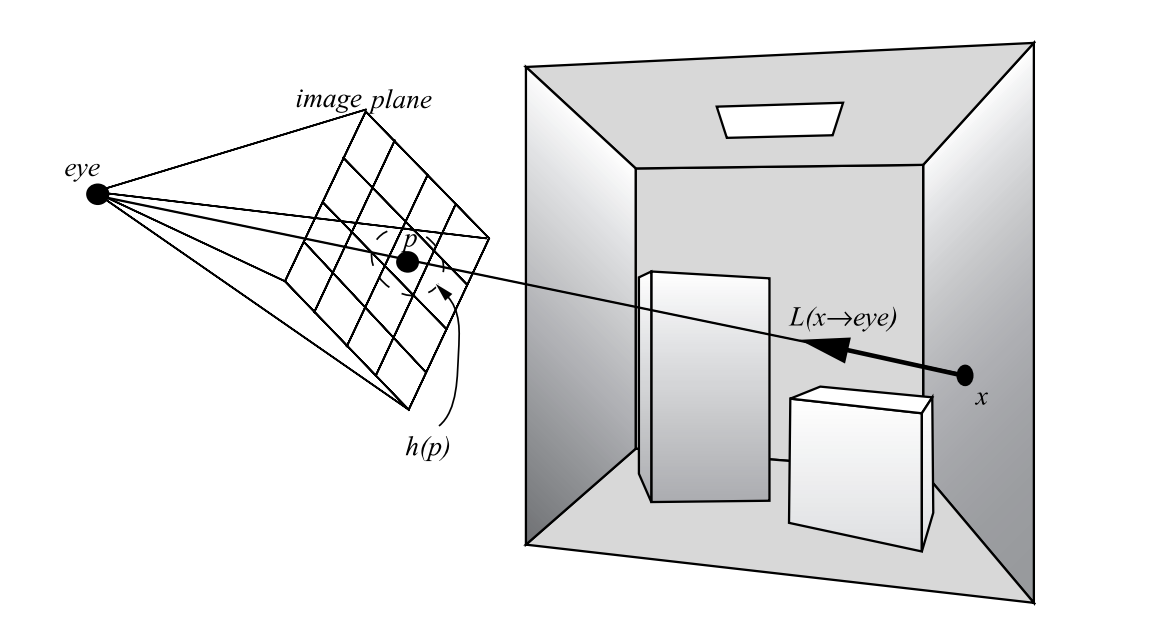
\includegraphics[scale=1]{obrazky-figures/ray_tracing_plane.png}
	\caption{3D mřížka. \textbf{Zdroj: \cite{advanced_global}}}
	\label{fig:3d_grid}
\end{figure}


Jak název napovídá, ray tracing používá paprsky k výpočtu barvy výsledného obrázku. Paprsek je polopřímka a je tedy definován počátečním bodem $\Vec{o}$ (origin) a směrem $\Vec{d}$ (direction). Nutnou funkcí pro funkčnost tohoto algoritmu je výpočet průsečíku paprsku s primitivy, pomocí kterých je scéna vytvořena. Možnosti výpočtu průsečíku paprsku s voxelem je popsána v sekci \ref{sec:voxel_intersection}. Jednoduchý ray tracing je popsán v algoritmu \ref{alg:rt_1}. Takto naivní implementace je samozřejmě velice neefektivní a pro běžně používané scény je nutné použít akcelerační struktury pro urychlení hledání průsečíku\cite{accelerated_rt}. Pro realistické zobrazování jsou krom primárních paprsků o paprsky sekundární. Tyto paprsky jsou použity například pro odrazy, refrakci a stíny.

Ve své standardní formě ray tracing neumožňuje generování měkkých stínů a spousty dalších sekundárních efektů.  Pro dosažení tíženého efektu lze využít například \textbf{Monte carlo ray tracing}(stochaistic ray tracing nebo distributed ray tracing) \cite{distributed_rt}. Namísto jediného paprsku pro výpočet stínů, odrazů a refrakcí je využito paprsků více a výsledky jejich výpočtu jsou následně průměrovány. Metoda umožňuje vytvoření mnoha dalších efektů, jako například hloubka pole, rozmazání pohybu atd.

\begin{center}
	\begin{czechalgorithm}[H] \label{alg:rt_1}
		ray = build\_ray(camera.position, image\_plane)

		min\_distance = MAX

		hit\_primitive = false

		\ForEach{\text{primitive in scene}} {

			(intersected, distance) = intersect(ray, primitive)

			\uIf{intersected \And distance < min\_distance}{

				hit\_primitive = primitive

				min\_distance = distance
			}
		}
		\caption{Ray tracing}
	\end{czechalgorithm}
\end{center}

\subsubsection{Ray marching}
Za zmínku stojí také algoritmus ray marching (sphere tracing). Namísto přímého výpočtu průsečíku se scénou - jak tomu je u spousty ray tracing implementací - postupuje paprsek ve scéně postupně, dokud nedojde k průsečíku.

Článek \cite{sphere_tracing} popisuje algoritmus následovně. Podmínkou funkčnosti algoritmu je mít možnost vypočítat z každého bodu ve scéně vzdálenost k jejímu povrchu. Pro tento účel lze využít takzvaných signed distance functions (SDF). Pro každý paprsek, kdy generování paprsků probíhá stejně jako u již zmíněného ray tracing, se iteruje napříč scénou dokud do ní paprsek nenarazí, nepřekoná maximální počet iterací či vykreslovací vzdálenost (algoritmus \ref{alg:ray_marching}).


\begin{center}
	\begin{czechalgorithm}[H] \label{alg:ray_marching}
		i = 0

		t = t\_min

		\While{t < t\_max \And i < MAX\_ITERATIONS}{

			distance\_to\_scene = dist\_func(ray)

			\uIf{distance < \varepsilon}{

				return t

			}
			t += distance\_to\_scene

			i += 1
		}
		return t\_max
		\caption{Ray marching}
	\end{czechalgorithm}
\end{center}

Pro tento algoritmus existuje značné množství optimalizací \cite{Keinert2014EnhancedST}. Jako je například 'over-relaxation', kdy dochází k zaměrně většímu kroku a případnému návratu zpět. Dalším příkladem je namísto sledování paprsku použít kužel, což značně snižuje množství iterací algoritmu.

\begin{figure}[H]
	\centering
	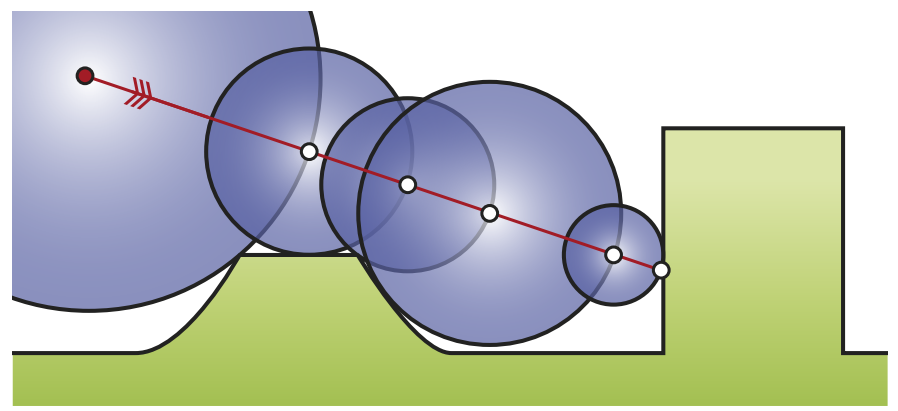
\includegraphics[scale=0.8]{obrazky-figures/ray_marching.png}
	\caption{Ray marching. \textbf{Zdroj: \cite{Keinert2014EnhancedST}}}
	\label{fig:ray_marching}
\end{figure}


\subsection{Radiozita}
Metody radiozity byly vyvinuty již v padesátých letech minulého století pro simulaci tepelného přenosu. Později byla popsána varianta pro vykreslování v článku \cite{radiosity}. Metoda je založena na jednoduchém principu; vzhledem k tomu, že každý povrch ve scéně může odrážet světlo, se dá tento povrch považovat za zdroj světla. Radiozita povrchu je dána rovnicí:


\begin{equation} \label{eq:voxel_coords}
	\begin{gathered}
		B_i = E_i + \rho_i \sum^N_{j = 1}B_jF_{ij} \text{ pro } i = 1 \text{ do } N
	\end{gathered}
\end{equation}

Kde $B$ je celkové množství energie vyzařované z povrchu, $E$ je množství energie vyzařované v povrchu bez vlivu okolí, $\rho$ je faktor reflexivity, $F$ je faktor určující jaká část energie dorazila na povrch a $N$ je počet povrchů ve scéně.

Z mého průzkumu vypadá, že je radiozita primárně používána pro předvýpočet globální iluminace v některých scénách a dále není počítána znova. Důvodem je pravděpodobně poměrně velká náročnost algoritmu.


\section{Voxel}
Jak uvádí kniha \cite{gfx_principles_practice}, voxel, nebo-li \textbf{vo}lume \textbf{el}ement, reprezentuje hodnotu na pravidelné mřížce ve 3D prostoru (obrázek \ref{fig:3d_grid}). Díky tomu, že je prostor rozdělen mřížkou pravidelně, lze voxel definovat pomocí třísložkového vektoru (rovnice \ref{eq:voxel_coords}). Pro účely vykreslování jsou voxelům přiřazovány další vlastnosti, jako například barva nebo materiál.

\begin{equation} \label{eq:voxel_coords}
	\begin{gathered}
		\vec{pozice_{voxel}} \in \mathbb{Z}_3
	\end{gathered}
\end{equation}

\begin{figure}[H]
	\centering
	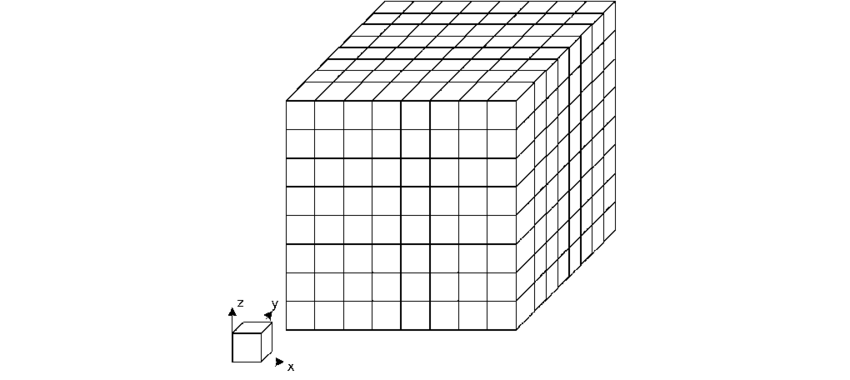
\includegraphics[scale=0.5]{obrazky-figures/3d_grid.png}
	\caption{3D mřížka. \textbf{Zdroj: }\url{https://www.researchgate.net/figure/The-three-dimensional-3D-Cartesian-grid-applied-on-the-simulation-domain-The-latter_fig1_234106571}}
	\label{fig:3d_grid}
\end{figure}

Voxely jsou často využívány v medicíně \cite{medical_vox}, například pro výstupy magnetické resonance (obrázek \ref{fig:mri_vox}).

\begin{figure}[H]
	\centering
	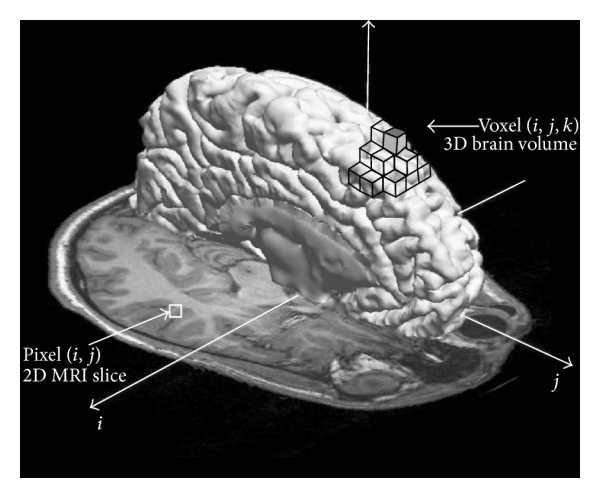
\includegraphics[scale=1]{obrazky-figures/voxel_mri.png}
	\caption{Zobrazení výsledku magnetické resonance pomocí voxelů. \textbf{Zdroj: \cite{mri}}}
	\label{fig:mri_vox}
\end{figure}

Dalším častým využitím je modelování terénu; Voxely přináší možnost reprezentovat převisy, čímž je terén značně realističtější, než při aplikaci často používaných výškových map. Pravděpodobně nejznámější software používající voxely pro terén je Minecraft (obrázek \ref{fig:minecraft}). Za zmínku stojí také hra Teardown (2020)\footnote{\url{https://www.teardowngame.com/}}, kde je celý herní svět vytvořen pomocí voxelů a umožňuje téměř neomezenou destrukci.

\begin{figure}[H]
	\centering
	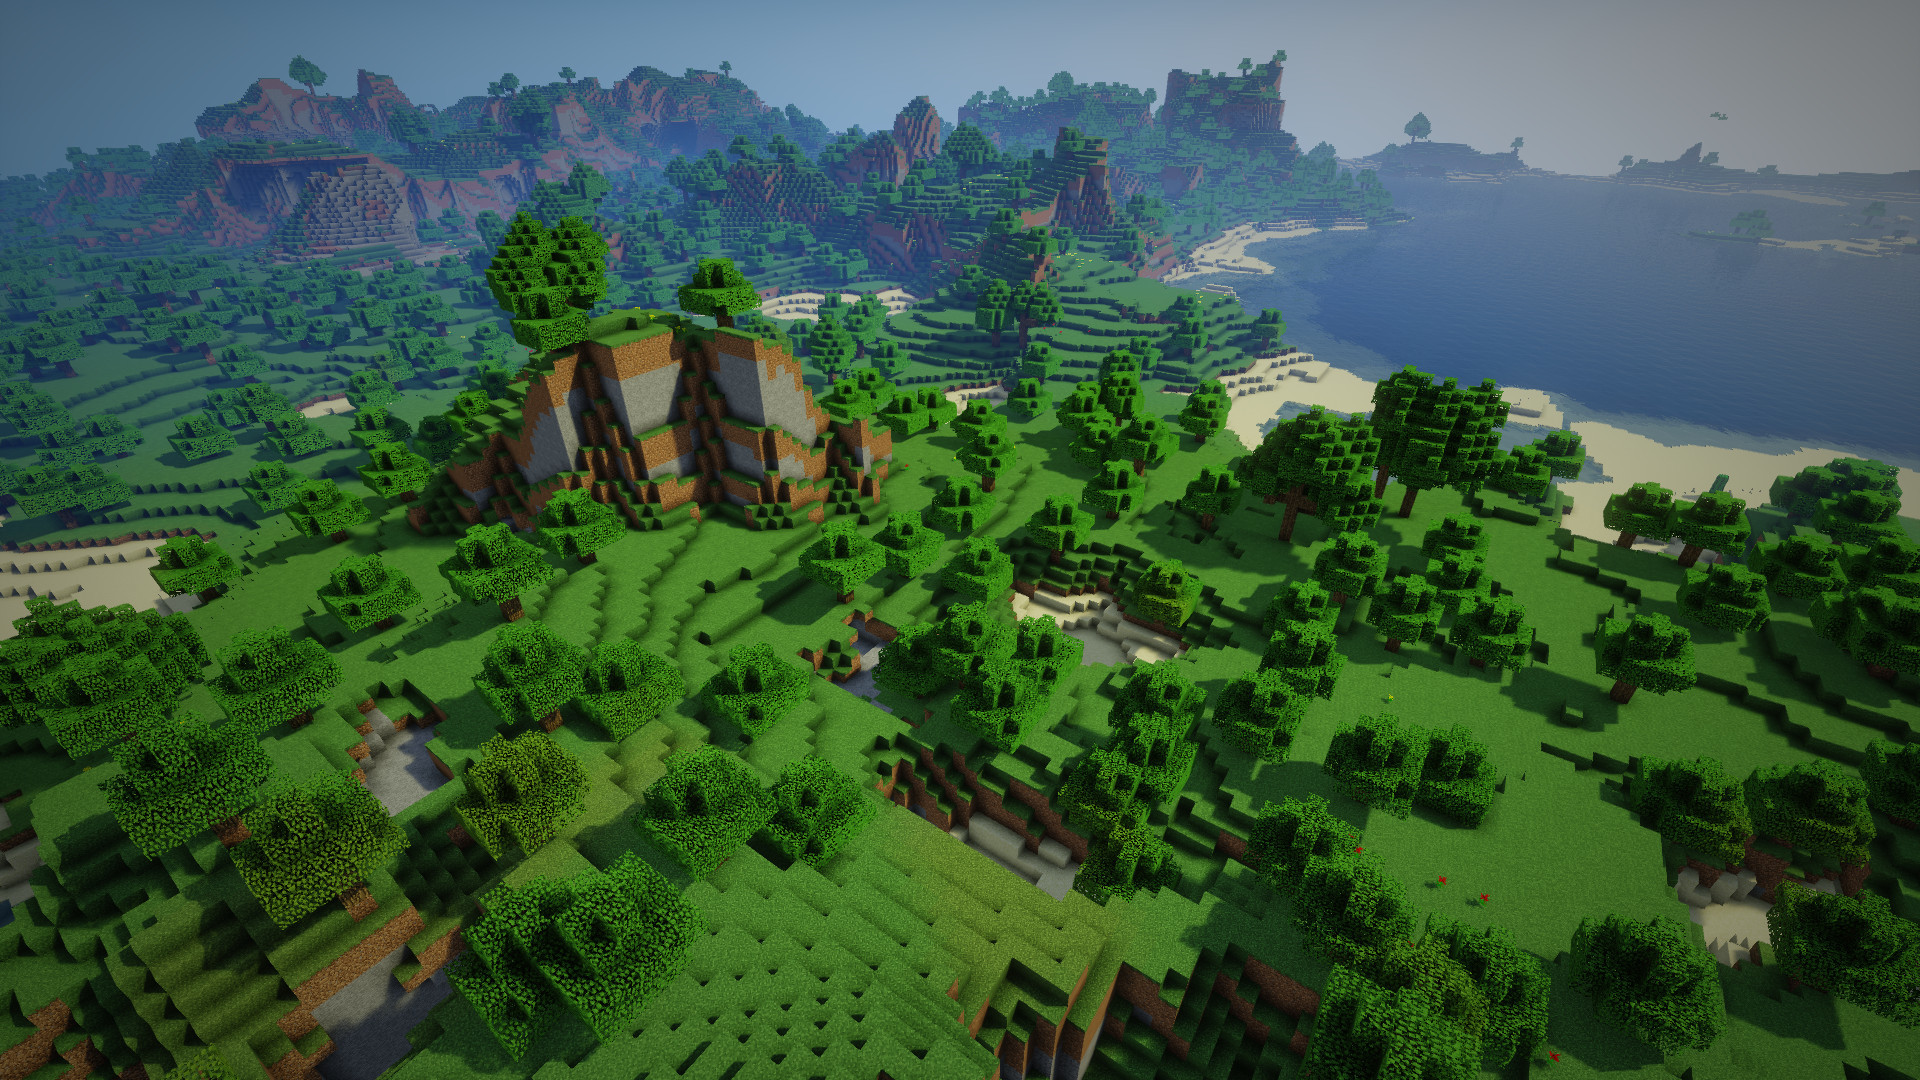
\includegraphics[scale=0.15]{obrazky-figures/minecraft.jpg}
	\caption{Minecraft. \textbf{Zdroj: \url{https://forums-cdn.spongepowered.org/uploads/default/original/2X/8/83abd20efc6cf5104c2f8c5459808bcd1addef7a.jpg}}}
	\label{fig:minecraft}
\end{figure}

\subsection{Vykreslování voxelových modelů}
Níže jsou popsány základní metody vykreslování voxelových modelů. Jedná se jen o základní příklady, ve skutečnosti existuje mnohem více metod, než by bylo rozumné zde popisovat.

\subsubsection{Rasterizace}
Pro vykreslování voxelových scén pomocí rasterizace je nutné ji převést na trojúhelníkovou reprezentaci. Toho se dá dosáhnout několika způsoby.

\paragraph{Instancované vykreslování} je velice primitivní metoda. Pro každý voxel, který je reprezentován přímo svojí pozicí a případně dalšími parametry (barva...), je vykreslena krychle o předem určené délce hran. Před samotným vykreslováním musí docházet k odstranění takových voxelů, které nejsou viditelné. Pokud by byl tento krok vynechán, bylo by vykreslování velice náročné. \cite{nousiainen_2019}

\begin{center}
	\begin{czechalgorithm}[H] \label{alg:instanced_cube}
		voxel\_array = cull\_voxels(all\_voxels)

		\ForEach{\text{voxel in voxel\_array}} {
			render\_cube(voxel.position)
		}
		\caption{Instancované vykreslování}
	\end{czechalgorithm}
\end{center}

\paragraph{Marching cubes \cite{marching_cubes}} je příkladem algoritmu pro extrakci povrchu z voxelových dat. Původně představen pro vizualizaci dat v medicínském odvětví, je současně využíván například pro vizualizaci terénu \cite{nguyen_2008}. Pro každou oblast v mřížce prostoru je zjištěno, který z rohů voxelu se nachází uvnitř či vně tělesa. Na základně toho je vypočten tvar a pozice generovaných trojúhelníků. V některých úpravách algoritmu je možné značně snížit počet vygenerovaných trojúhelníků a snížení redundantnosti dat. Po vygenerování často dochází k minimalizaci počtu trojúhelníku. Následuje zjednodušená verze algoritmu.

\begin{center}
	\begin{czechalgorithm}[H] \label{alg:marching_cubes}
		\ForEach{voxel in area} {
			case = calculate\_case(voxel)

			triangles = generate\_triangles(voxel.position, case)

			result.add(triangles)

		}
		\caption{Marching cubes}
	\end{czechalgorithm}
\end{center}

Existují další metody, jako například \textbf{marching tetrahedra}, ale tato práce rasterizačních metod nevyužívá a proto tu nebudou dále zmiňovány.

\subsubsection{Ray casting} \label{sec:voxel_intersection}
Při vykreslování pomocí paprsků lze problém rozdělit na dvě části. První z nich je výpočet průsečíku s voxelem a druhým je využití hierarchické struktury pro minimalizaci počtu navštívených voxelů. Hierarchické struktury jsou v samostatné sekci.

\paragraph{Průsečík paprsku s voxelem} lze počítat mnoha způsoby. Primitivní přístup k řešení tohoto problému je počítat průsečík s každou rovinou, která reprezentuje voxel a následně vybrat ten nejbližší (algoritmus \ref{alg:ray_box_primitive}). Tohle řešení je ale poněkud náročné a využívá podmínky, což může podle článku \cite{gpu_branch} značně zpomalit výpočet.

\begin{center}
	\begin{czechalgorithm}[H] \label{alg:ray_box_primitive}
		corner_1 = voxel.position

		corner_2 = voxel.position + voxel\_length

		coeffs[0] = (corner_1.x - ray.origin.x) / ray.direction.x

		coeffs[1] = (corner_1.y - ray.origin.y) / ray.direction.y

		coeffs[2] = (corner_1.z - ray.origin.z) / ray.direction.z

		coeffs[3] = (corner_2.x - ray.origin.x) / ray.direction.x

		coeffs[4] = (corner_2.y - ray.origin.y) / ray.direction.y

		coeffs[5] = (corner_2.z - ray.origin.z) / ray.direction.z

		hit = false

		distance = \inf

		\ForEach{\text{coef in coefs}} {

			\uIf {coef >= 0} {
				hit = true

				hit\_point = ray.origin + ray.direction * coef;

				\uIf{is\_in\_box\_bounds(corner_1, hit\_point)}{

					distance = coef;
				}
			}
		}
		\caption{Primitivní výpočet průsečíku s voxelem}
	\end{czechalgorithm}
\end{center}

Vhodnější alternativou pro výpočet průsečíku paprsku s voxelem lze najít v publikaci \cite{efficient_box_intersect}. Tato metoda využívá dlaždic (slabs), kdy je voxel považován za průsečík tří z nich. Na obrázku \ref{fig:slabs} je vizualizace výpočtu ve 2D - ve 3D je výpočet obdobný. Algoritmus pro 2D je popsán v rovnici \ref{eq:slabs}.


\begin{equation} \label{eq:slabs}
	\begin{gathered}
		x_{min} = p_x + t_{xmin} d_x\\
		t_{xmin} = \frac{(x_{min} - p_x)}{d_x}\\
		\\
		y_{min} = p_y + t_{ymin} d_y\\
		t_{ymin} = \frac{(y_{min} - p_y)}{d_y}\\
		\\
		t_{xenter} = \min(t_{xmin}, t_{xmax})\\
		t_{xexit} = \max(t_{xmin}, t_{xmax})\\
		\\
		t_{yenter} = \min(t_{ymin}, t_{ymax})\\
		t_{yexit} = \max(t_{ymin}, t_{ymax})\\
		\\
		t_{exter} = \max(t_{xenter}, t_{yenter})\\
		t_{exit} = \min(t_{xexit}, t_{yexit})\\
	\end{gathered}
\end{equation}

\begin{figure}[H]
	\centering
	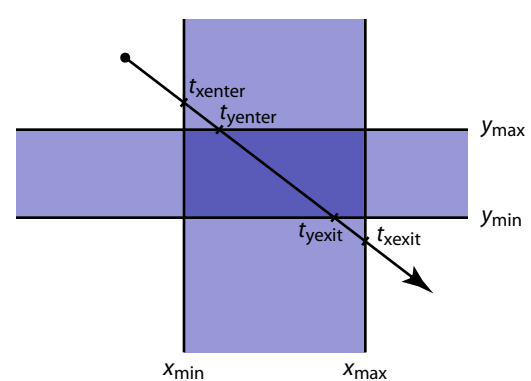
\includegraphics[scale=1.3]{obrazky-figures/slab_intersect.png}
	\caption{Průsečík s voxelem metodou dlaždic. \textbf{Zdroj: \cite{Cunha13}}}
	\label{fig:slabs}
\end{figure}


\subsection{Používané formáty}
Pro ukládání voxelových scén existuje poměrně velké množství formátů. Bohužel neexistuje žádný standardizovaný formát, i když nějaké pokusy o to již byly (například VolDat\footnote{http://www.volumesoffun.com/voldat-format/}). Následuje popis vybraných formátů.

\paragraph{Vox} formát byl vytvořen pro aplikaci MagicaVoxel\footnote{\url{http://ephtracy.github.io/}}, což je modelovací software pro voxelové scény. Jedná se o binární formát, kde jsou barvy zakódovány pomocí palety. Také podporuje různé typy materiálů. Jelikož MagicaVoxel nepodporuje větší modely než 256x256x256 voxelů, zpravidla v tomto formátu větší scény nejsou. Specifikace formátu jsou v \cite{vox_format}.

\paragraph{SVX} (Simple Voxels) je archivový formát. Archiv obsahuje soubor manifest.xml, který popisuje velikost mřížky, velikost voxelů, paletu materiálů a další metadata. Samotné voxely jsou popsány pomocí obrázků v jednokanálovém formátu PNG, přičemž každý pixel slouží jako odkaz do palety modelů. Tento formát je používán především pro 3D tisk. Specifikaci formátu najdete na \cite{svx_format_2014}.

Existuje spousta dalších formátů, značné množství pro 3D tisk, ale také pro využití v medicíně, jak již bylo zmíněno dříve. Dle mého průzkumu je nejčastějším přístupem při volbě formátu pro vykreslovací engine vytvořit formát vlastní.


\section{Hierarchické struktury}


Akceleracni struktury

- zadne

- grid

- octree/svo

GPU vulkan

- co je akcelerace na gpu

- pipelines

\chapter{Návrh řešení}
\label{navrh}
oduvodneni SVO

popis ray casting algoritmu

popis light field probes

\chapter{Implementace}
\label{implementace}
nacitani a tvorba SVO


\chapter{Testování a vyhodnocení}
\label{testovani}
udelat graf podle poctu voxelu nebo neco

pametova narocnost

\chapter{Další práce}
\label{dalsi_prace}
co je potreba nacit/dodelat


\chapter{Závěr}
\label{zaver}




%===============================================================================
